\section{Geometric Location}
\label{sec:geo}

Geometric localization aims to pinpoint the target. This can be done either by 
inferring relative spacial relationship to beacons or fingerprints, or dead-reckoning
with IMU sensors. Statistic models, such as Kalman Filter and Particle Filter, 
enable us to calculate posterior distribution of geometric locations from various observations.
In this section, we discuss how Drummer use Exponential Sine Sweep (ESS) method to measure 
distance to nearest surfaces, such as walls. We argue that these distances provide positive calibration 
information to geometric localizations.


\subsection{Exponential Sine Sweep Method}

The goal in Drummer is to measure distances from target phone to nearby walls, ceiling, or floor.
%An indoor environment is commonly regarded as linear and time-invariant system to acoustic signal.
It is ideal to measure these distances by looking at the acoustic impulse response at the location of 
the phone, and search for spikes in echoes to infer distances to walls. 
To achieve this, we employ the Exponential Sine Sweep (ESS)
method proposed by Farina \cite{farina2000simultaneous}. 


We briefly introduce the method here. The first step is to generate an ESS signal:
\begin{equation}
x(t) = \sin \left(\frac{\omega_1 \cdot T}{\ln \left(\frac{\omega_2}{\omega_1}\right)} \cdot \left(e^{\frac{t}{T} \cdot \ln \left(\frac{\omega_2}{\omega_1}\right)} - 1 \right)\right)
\end{equation}
, starting from frequency $\omega_1$ and ending at frequency $\omega_2$, with duration $T$ seconds. 
The generated ESS signal is sent to smart phone speaker. The sound generated by speaker and echoes are
recorded by one microphone of the smart phone, denoted as $y(t)$.  
We model $y(t)$ as sum of response signal of $x(t)$ and noise signal $n(t)$:
\begin{equation}
y(t) = F[x(t)] + n(t)
\end{equation}
. Because indoor environments are seen as a single-input, single-output, linear, and time invariant system, whose impulse 
response is denoted as $h(t)$, we can rewrite $F[x(t)]$ as convolution of $x(t)$ and $h(t)$:
\begin{equation}
y(t) = x(t) \ast h(t) + n(t)
\end{equation}


Our goal is to deconvolve and get $h(t)$ from $y(t)$ and $x(t)$. An inverse filter $f(t)$, which is the reversed $x(t)$ along
time axis, can be used to pack $x(t)$ to a nearly Dirac's delta function $\delta(t)$:
\begin{equation}
\delta(t) = x(t) \ast f(t)
\end{equation}
. So we can get $h(t)$ by convolving recorded sound $y(t)$ with inverse filter $f(t)$:
\begin{equation}
h(t) = y(t) \ast f(t)
\end{equation}


In a later work \cite{farina2007advancements}, Farina discussed the pros and cons of this method. 
It has better noise rejection than same length Maximum Length Sequence (MLS), and doesn't require 
time synchronization. The generated impulse will delay on the original signal, but it will 
have little influence to our result, as 
we are only looking at the time difference between the impulse and its echoes. 
And other downsides of this approaches are also irrelevant if we are only looking at echoes. \fxnote{better argument/ desc here}




\subsection{Practical Constrains}

There are several practical constrains when applying this approach on commercial smart phone for distance measurement. 
Firstly, smart phones speakers are mostly used for audible sound, so their frequency range will be limited on both ends. 
%A usual smart phone speaker has 30Hz-20000Hz frequency range.
Secondly, smart phone speakers will have non-flat frequency response. So the generated ESS signal will 
have different amplitude at different frequencies. Finally, the sound cannot be loud or long.



good audio chips are coming out:  http://goo.gl/lYqdX8


\subsection{How the result can be used?}

True positive is high, so it can only be used for calibration.


several sample

% \subsection{Distance from Nearest Walls}

% Geometric information can be obtained from measuring Round Trip Time (RTT)
% of a probing chirp. 

% \subsubsection{Chirp}


% sweep frequency chirp


% Select Chirp Amplitude and Frequency

% We firstly measure the ambient sound, and choose a quiet frequency.


% What is chirp


% why chirp?


% How to generate chirp?


% What chirp to use?


% How to see echo? Time delay of echo, Shape of echo pulse, Phase Diff


% SNR etc.

% \fxnote{GRAPH: chirp and echo shape}

% \subsubsection{Recording}

% \subsubsection{Cross-correlation and Audio Reduction}

% After receiving the original sound and echo, we do auto-correlation with original sound,
% and remove it from the audio track.

% \fxnote{GRAPH: how auto-correlation works}


% \subsubsection{Locating Echoes}

% Envelop is the sound of big surface. Physical explanation. 
% Define envelop as the same duration of original sound.



% \begin{figure}[H]
% \centering
% 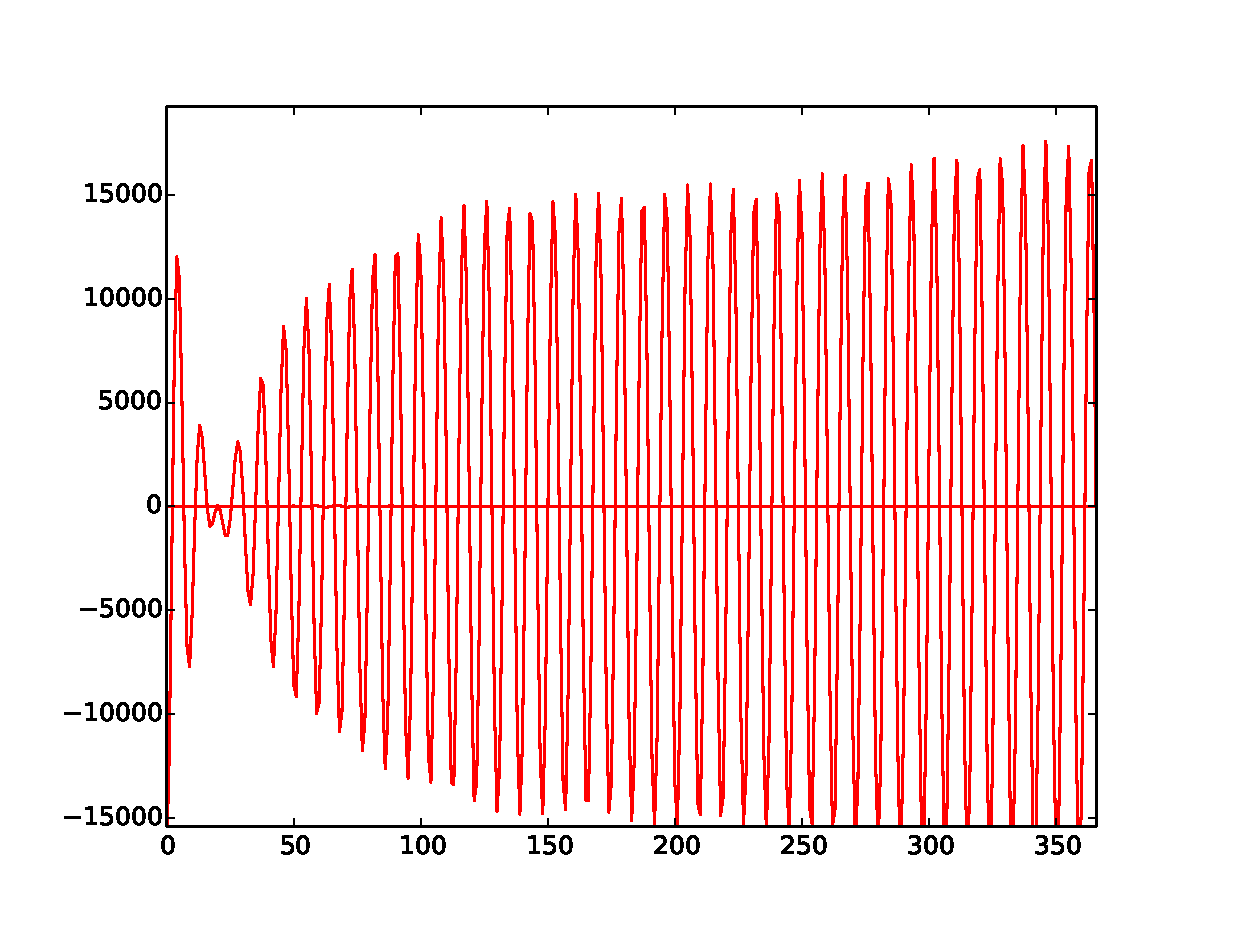
\includegraphics[width=0.45\textwidth]{./fig/20cm.eps}
% \caption{20cm from wall, 50ms chirp}
% \end{figure}

% \begin{figure}[H]
% \centering
% 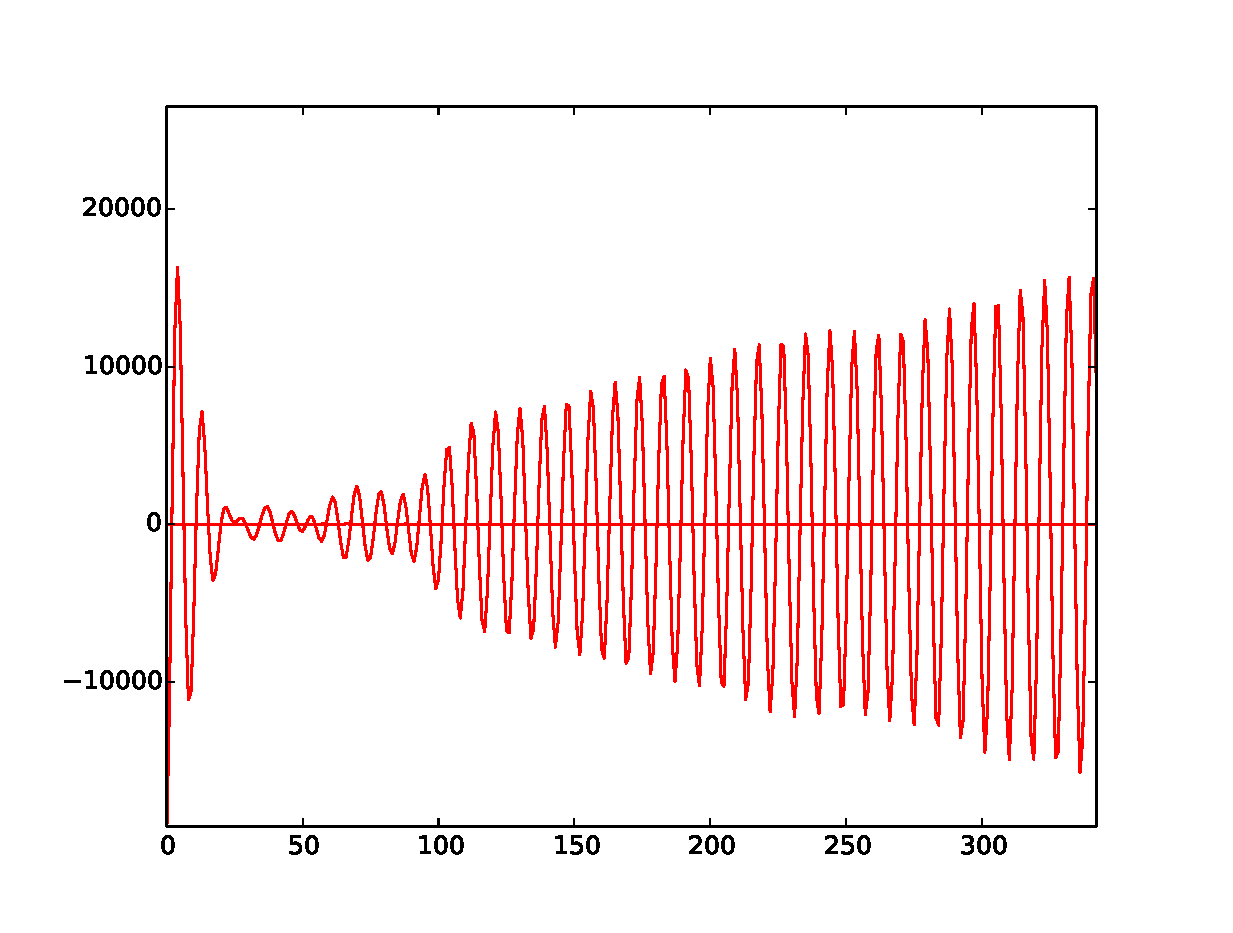
\includegraphics[width=0.45\textwidth]{./fig/40cm.eps}
% \caption{40cm from wall, 50ms chirp}
% \end{figure}

% \begin{figure}[H]
% \centering
% 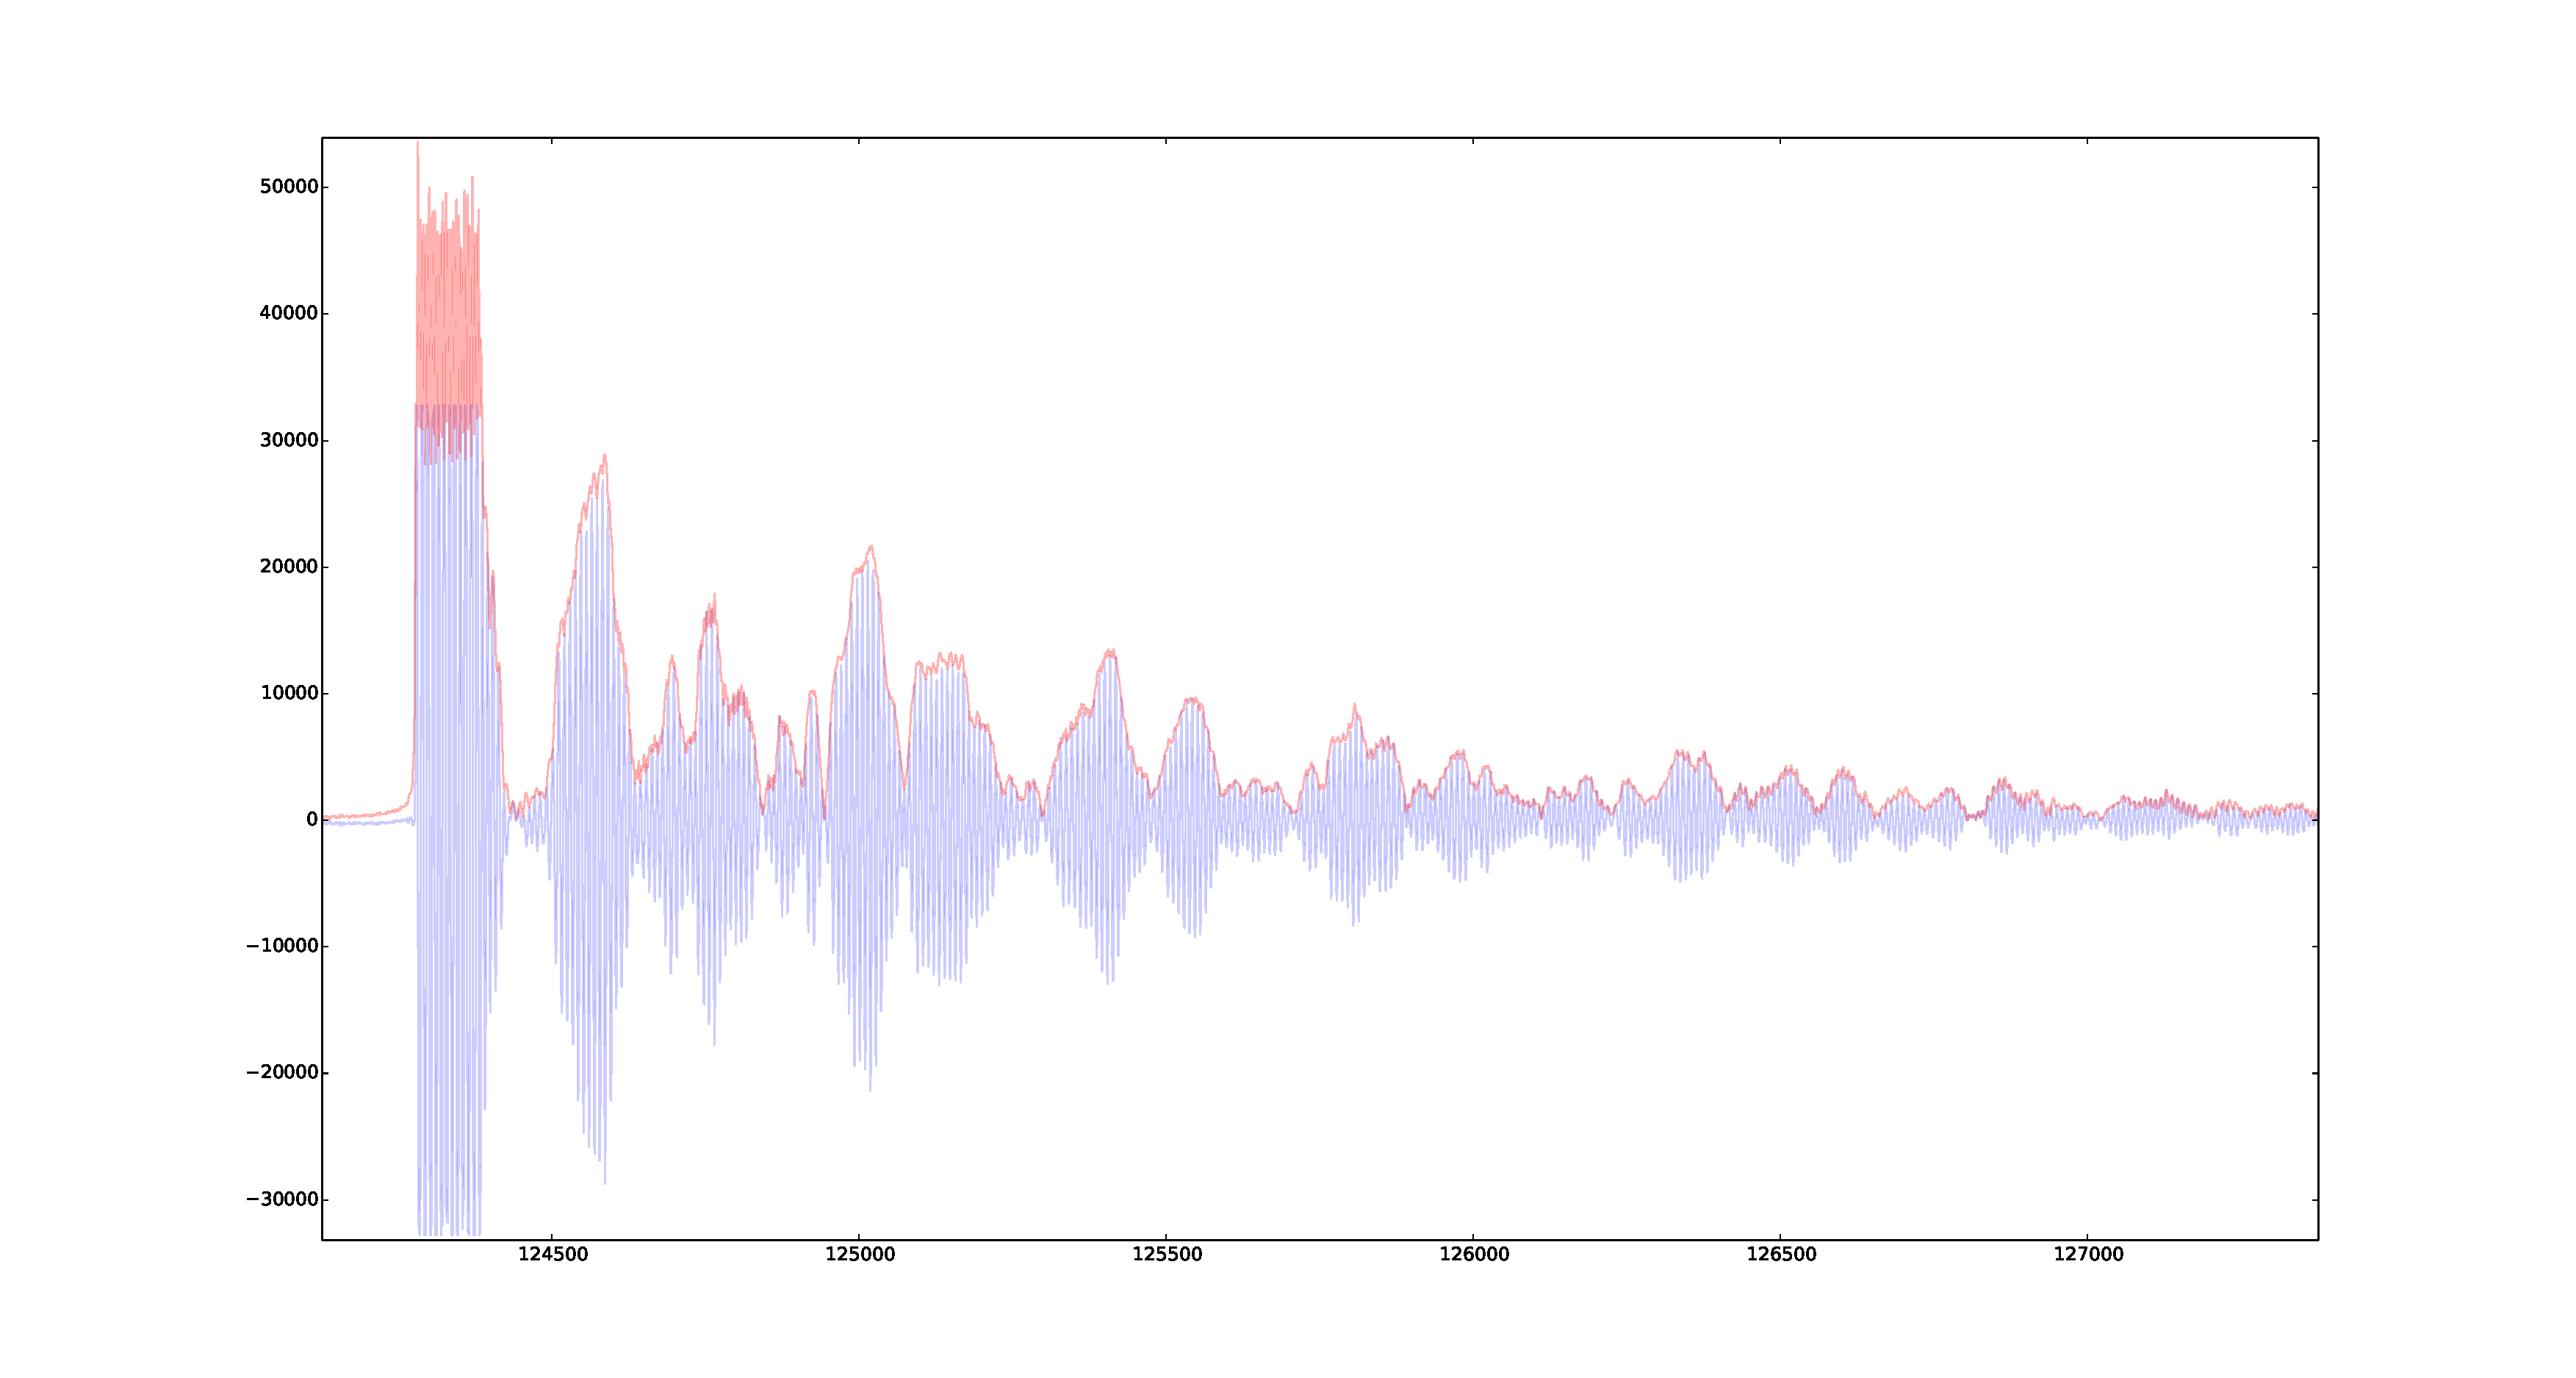
\includegraphics[width=0.45\textwidth]{./fig/inroom.pdf}
% \caption{40cm from wall, 5ms chirp}
% \end{figure}



% % \subsubsection{Phase Diff}



% % \subsubsection{Shape of Echo}


% % \subsubsection{Iterative Audio Reduction}

% % We remove the acoustic effects of an object after determining its existence, and 
% % in turn investigate the remaining sound iteratively. 


% \subsection{Orientations of All Echoes}

% We use TDoA of envelops to different microphones to determine the direction 
% of the object represented by the envelop.


% Binaural beat


